\documentclass[12pt, a4paper, oneside, openright, titlepage]{book}
\usepackage[utf8]{inputenc}
\raggedbottom
%%%%%%%%%%%%%%%%% Book Formatting Comments:

%%%%%%%%%%%%%%%%%%%%%%%%%%%%%%%%%%%%% for Part

%%%%%%%%%%%%%%%%%%%%%% for chapter

%%%%%%%%%%%%%%%%%%%% for section




%%%%%% PACKAGES %%%%%%%
\usepackage{hyperref}
\hypersetup{
    colorlinks,
    citecolor=black,
    filecolor=black,
    linkcolor=black,
    urlcolor=black
}
\usepackage{amsmath} % Math display options
\usepackage{amssymb} % Math symbols
%\usepackage{amsfonts} % Math fonts
%\usepackage{amsthm}
\usepackage{mathtools} % General math tools
\usepackage{array} % Allows you to write arrays
\usepackage{empheq} % For boxing equations
% \usepackage{mathabx}
% \usepackage{mathrsfs}
\usepackage{nameref}
\usepackage{wrapfig}

\usepackage{soul}
\usepackage[normalem]{ulem}

\usepackage{txfonts}
\usepackage{cancel}
\usepackage[toc, page]{appendix}
\usepackage{titletoc,tocloft}
\setlength{\cftchapindent}{1em}
\setlength{\cftsecindent}{2em}
\setlength{\cftsubsecindent}{3em}
%\setlength{\cftsubsubsecindent}{4em}
\usepackage{titlesec}

%\titleformat{\section}
%  {\normalfont\fontsize{25}{15}\bfseries}{\thesection}%{1em}{}
%\titleformat{\section}
%  {\normalfont\fontsize{20}{15}\bfseries}%{\thesubsection}{1em}{}
%\setcounter{secnumdepth}{1}  
  
  

%\newcommand\numberthis{\refstepcounter{equation}\tag{\theequation}} % For equation labelling
\usepackage[framemethod=tikz]{mdframed}

\usepackage{tikz} % For drawing commutative diagrams
\usetikzlibrary{cd}
\usetikzlibrary{calc}
\tikzset{every picture/.style={line width=0.75pt}} %set default line width to 0.75p

\usepackage{datetime}
\usepackage[margin=1.5in]{geometry}
\setlength{\parskip}{1em}
\usepackage{makeidx}         % allows index generation
\usepackage{graphicx}       % standard LaTeX graphics tool
\usepackage{multicol}        % used for the two-column index
\usepackage[bottom]{footmisc}% places footnotes at page bottom

\usepackage{newtxtext}       % 
\usepackage{newtxmath}       % selects Times Roman as basic font
\usepackage{float}
\usepackage{fancyhdr}
\setlength{\headheight}{15pt} 
\pagestyle{fancy}
\lhead[\leftmark]{}
\rhead[]{\leftmark}

%\usepackage{enumitem}

\usepackage{url}
\allowdisplaybreaks

%%%%%% ENVIRONMENTS %%%
\definecolor{purp}{rgb}{0.29, 0, 0.51}
\definecolor{bloo}{rgb}{0, 0.13, 0.80}



%%\newtheoremstyle{note}% hnamei
%{3pt}% hSpace above
%{3pt}% hSpace belowi
%{}% hBody fonti
%{}% hIndent amounti
%{\itshape}% hTheorem head fonti
%{:}% hPunctuation after theorem headi
%{.5em}% hSpace after theorem headi
%{}% hTheorem head spec (can be left empty, meaning ‘normal’)i





% %%%%%%%%%%%%% THEOREM DEFINITIONS

\spnewtheorem{axiom}{Axiom}[chapter]{\bfseries}{\itshape}


\spnewtheorem{construction}{Construction}[chapter]{\bfseries}{\itshape}

\spnewtheorem{props}{Properties}[chapter]{\bfseries}{\itshape}


\renewcommand{\qedsymbol}{$\blacksquare$}


\numberwithin{equation}{section}

\newenvironment{qest}{
    \begin{center}
        \em
    }
    {
    \end{center}
    }

%%%%%% MACROS %%%%%%%%%
%% New Commands
\newcommand{\ip}[1]{\langle#1\rangle} %%% Inner product
\newcommand{\abs}[1]{\lvert#1\rvert} %%% Modulus
\newcommand\diag{\operatorname{diag}} %%% diag matrix
\newcommand\tr{\mbox{tr}\.} %%% trace
\newcommand\C{\mathbb C} %%% Complex numbers
\newcommand\R{\mathbb R} %%% Real numbers
\newcommand\Z{\mathbb Z} %%% Integers
\newcommand\Q{\mathbb Q} %%% Rationals
\newcommand\N{\mathbb N} %%% Naturals
\newcommand\F{\mathbb F} %%% An arbitrary field
\newcommand\ste{\operatorname{St}} %%% Steinberg Representation
\newcommand\GL{\mathbf{GL}} %%% General Linear group
\newcommand\SL{\mathbf{SL}} %%% Special linear group
\newcommand\gl{\mathfrak{gl}} %%% General linear algebra
\newcommand\G{\mathbf{G}} %%% connected reductive group
\newcommand\g{\mathfrak{g}} %%% Lie algebra of G
\newcommand\Hbf{\mathbf{H}} %%% Theta fixed points of G
\newcommand\X{\mathbf{X}} %%% Symmetric space X
\newcommand{\catname}[1]{\normalfont\textbf{#1}}
\newcommand{\Set}{\catname{Set}} %%% Category set
\newcommand{\Grp}{\catname{Grp}} %%% Category group
\newcommand{\Rmod}{\catname{R-Mod}} %%% Category r-modules
\newcommand{\Mon}{\catname{Mon}} %%% Category monoid
\newcommand{\Ring}{\catname{Ring}} %%% Category ring
\newcommand{\Topp}{\catname{Top}} %%% Category Topological spaces
\newcommand{\Vect}{\catname{Vect}_{k}} %%% category vector spaces'
\newcommand\Hom{\mathbf{Hom}} %%% Arrows

\newcommand{\map}[2]{\begin{array}{c} #1 \\ #2 \end{array}}

\newcommand{\Emph}[1]{\textbf{\ul{\emph{#1}}}}




%% Math operators
\DeclareMathOperator{\ran}{Im} %%% image
\DeclareMathOperator{\aut}{Aut} %%% Automorphisms
\DeclareMathOperator{\spn}{span} %%% span
\DeclareMathOperator{\ann}{Ann} %%% annihilator
\DeclareMathOperator{\rank}{rank} %%% Rank
\DeclareMathOperator{\ch}{char} %%% characteristic
\DeclareMathOperator{\ev}{\bf{ev}} %%% evaluation
\DeclareMathOperator{\sgn}{sign} %%% sign
\DeclareMathOperator{\id}{Id} %%% identity
\DeclareMathOperator{\supp}{Supp} %%% support
\DeclareMathOperator{\inn}{Inn} %%% Inner aut
\DeclareMathOperator{\en}{End} %%% Endomorphisms
\DeclareMathOperator{\sym}{Sym} %%% Group of symmetries


%% Diagram Environments
\iffalse
\begin{center}
    \begin{tikzpicture}[baseline= (a).base]
        \node[scale=1] (a) at (0,0){
          \begin{tikzcd}
           
          \end{tikzcd}
        };
    \end{tikzpicture}
\end{center}
\fi




\newdateformat{monthdayyeardate}{%
    \monthname[\THEMONTH]~\THEDAY, \THEYEAR}
%%%%%%%%%%%%%%%%%%%%%%%

\newcommand{\mb}[1]{\mathbf{#1}}

%%%%%% BEGIN %%%%%%%%%%


\begin{document}

%%%%%% TITLE PAGE %%%%%

\begin{titlepage}
    \centering
    \scshape
    \vspace*{\baselineskip}
    \rule{\textwidth}{1.6pt}\vspace*{-\baselineskip}\vspace*{2pt}
    \rule{\textwidth}{0.4pt}
    
    \vspace{0.75\baselineskip}
    
    {\LARGE Linear Algebra: A complete Guide}
    
    \vspace{0.75\baselineskip}
    
    \rule{\textwidth}{0.4pt}\vspace*{-\baselineskip}\vspace{3.2pt}
    \rule{\textwidth}{1.6pt}
    
    \vspace{2\baselineskip}
    Linear Algebra \\
    \vspace*{3\baselineskip}
    \monthdayyeardate\today \\
    \vspace*{5.0\baselineskip}
    
    {\scshape\Large Elijah Thompson, \\ Physics and Math Honors\\}
    
    \vspace{1.0\baselineskip}
    \textit{Solo Pursuit of Learning}
    \vfill
    \enlargethispage{1in}
    \begin{figure}[b!]
    \makebox[\textwidth]{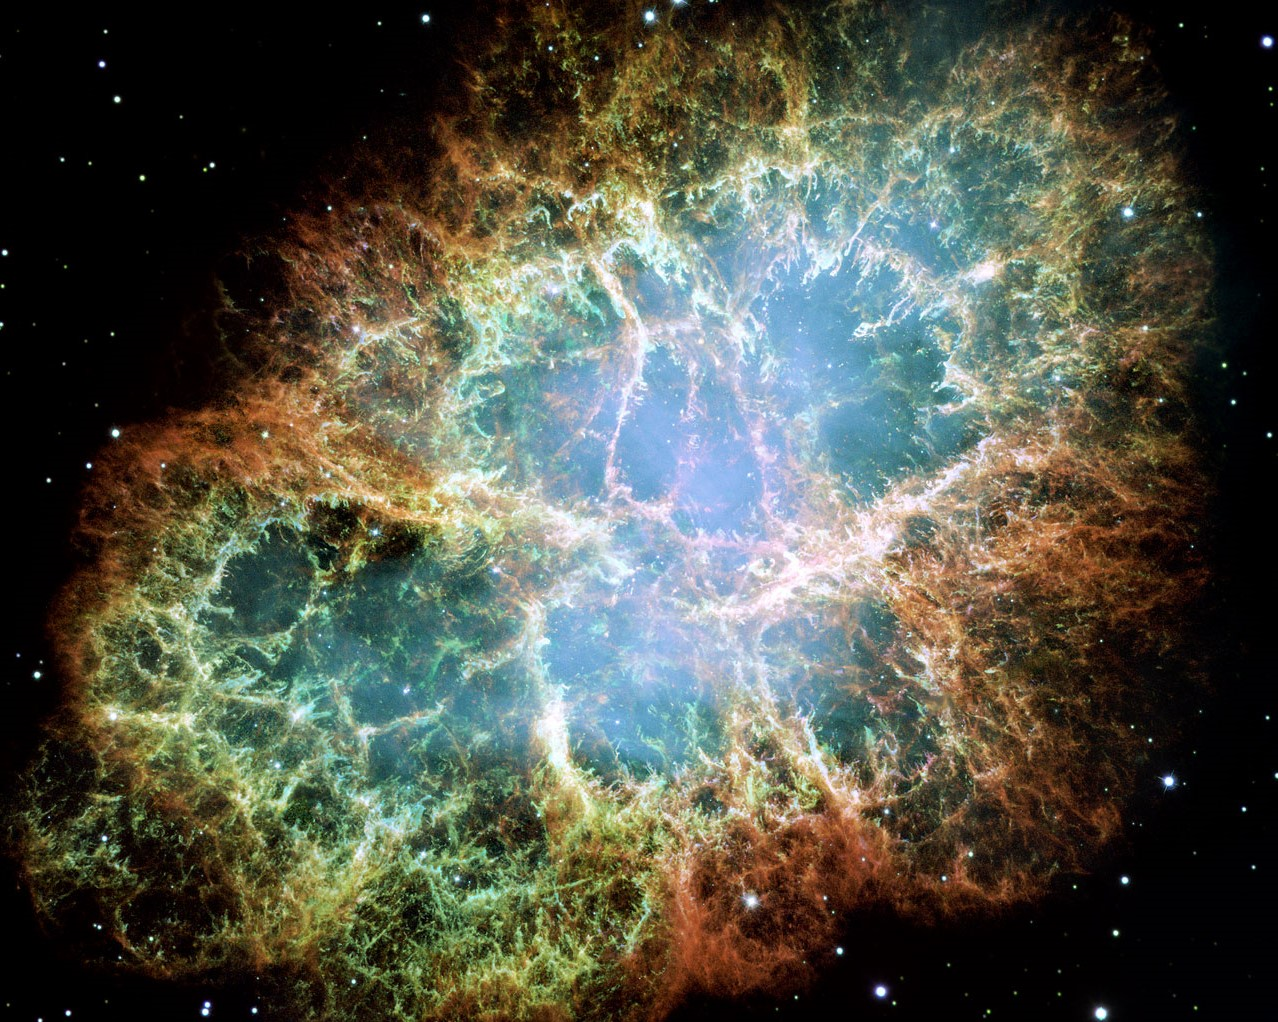
\includegraphics[width=\paperwidth, height =10cm]{../../Crab.jpg}}
    \end{figure}
\end{titlepage}

%%%%%%%%%%%%%%%%%%%%%%%
\tableofcontents

%%%%%%%%%%%%%%%%%%%%%%%%%%%%%%%%%%%%% - Part 1
\part{Vector Space Theory}

%%%%%%%%%%%%%%%%%%%%%% - P1.Chapter 1
\chapter{Vector Spaces}


\begin{subappendices}
    \section{Constructions}
\end{subappendices}

%%%%%%%%%%%%%%%%%%%%%% - P1.Chapter 2
\chapter{Linear Maps}




%%%%%%%%%%%%%%%%%%%%%% - P1.Chapter 3
\chapter{Matrix Operations}



%%%%%%%%%%%%%%%%%%%%%% - P1.Chapter 4
\chapter{Determinants}



%%%%%%%%%%%%%%%%%%%%%% - P1.Chapter 5
\chapter{Spectral Theory}



%%%%%%%%%%%%%%%%%%%%%% - P1.Chapter 6
\chapter{Canonical Forms}

\section{Triangular Form}

In this section we aim to construct the triangular form of linear maps, and demonstrate some properties this canonical form has. Throughout this section we presume $V$ to be a finite-dimensional vector space over a field $\F$. 


One important result we aim to show is that the matrix of a linear operator $T:V \rightarrow V$ with respect to a basis $\beta = \{\mb x_1,...,\mb x_n\}$, $[T]_{\beta}^{\beta}$, is in upper triangular form if and only if $T(W_i) \subseteq W_i$ for all $W_i = \spn(\mb x_1,...,\mb x_i)$.

\begin{defn}[Invariant Subspaces]
    Let $T:V \rightarrow V$ be a linear mapping. A subspace $W \subseteq V$ is said to be \emph{invariant} under $T$ if $T(W) \subseteq W$.
\end{defn}

\begin{eg}
    \begin{enumerate}[label = \alph*]
        \item $\{\mb 0\}$ and $V$ are invariant under all linear mappings $T:V\rightarrow V$
        \item $\ker(T)$ and $\ran(T)$ are invariant subspaces for all $T$ as well
        \item If $\lambda$ is an eigenvector of $T$ then the eigenspace $E_{\lambda}$ is invariant under $T$
    \end{enumerate}
\end{eg}

\begin{prop}
    Let $V$ be a vector space, let $T:V\rightarrow V$ be a linear mapping, and let $\beta = \{\mb x_1,...,\mb x_n\}$ be a basis for $V$. Then $[T]_{\beta}^{\beta}$ is upper-triangular if and only if each of the subspaces $W_i = \spn(\{\mb x_1,..., \mb x_i\})$ is invariant under $T$. Note that $$\{\mb 0\} \subset W_1 \subset W_1 \subset ... \subset W_{n-1} \subset W_n = V$$
\end{prop}

\begin{defn}
    We say that a linear mapping $T:V \rightarrow V$ on a finite-dimensional vector space $V$ is triangularizable if there exists a basis $\beta$ such that $[T]_{\beta}^{\beta}$ is upper triangular.
\end{defn}


\begin{rmk}
    To show that a mapping is triangularizable we must produce the increasing sequence of invariant subspaces $$\{\mb 0\} \subset W_1 \subset W_1 \subset ... \subset W_{n-1} \subset W_n = V$$
    spanned by the subsets of the basis $\beta$ and show that each $W_i$ is invariant under $T$.
\end{rmk}


\begin{prop}
    Let $T:V\rightarrow V$ and let $W \subset V$ be an invariant subspace. Then the characteristic polynomial of the restriction $T\rvert_W$ divides the characteristic polynomial of $T$.
\end{prop}

\begin{proof}
    Let $\alpha = \{\mb x_1,...,\mb x_k\}$ be a basis for $W$, and extend $\alpha$ to a basis $\beta = \{\mb x_1,...,\mb x_k,...,\mb x_n\}$ of $V$. Since $W$ is invariant under $T$, for each $i \leq k$ we have $$T(\mb x_i) = a_{1i}\mb x_1 + ... + a_{ki}\mb x_k + 0\mb x_{k+1} + ... + 0 \mb x_n$$
    Hence, the matrix $[T]_{\beta}^{\beta}$ has a block form composition $$[T]_{\beta}^{\beta} = \begin{bmatrix} A & B \\ 0 & C \end{bmatrix}$$
    where $A = [T\rvert_W]_{\alpha}^{\alpha}$ is a $k \times k$ matrix. When we compute the characteristic polynomial of $T$ using this matrix, we have $\det(T - \lambda I) = \det(A - \lambda I)\det(C - \lambda I)$ where $\det(A - \lambda I)$ is the characteristic polynomial of $T\rvert_W$, as desired.
\end{proof}


\begin{thm}
    Let $V$ be a finite-dimensional vector space over a field $\F$, and let $T:V\rightarrow V$ be a linear mapping. Then $T$ is triangularizable if and only if the characteristic polynomial equation of $T$ has $dim(V)$ roots (counted with multiplicities) in the field $F$.
\end{thm}

\begin{lem}
    Let $T:V\rightarrow V$ be as in the theorem, and assume that the characteristic polynomial of $T$ has $n = dim(V)$ roots in $\F$. If $W \subsetneq V$ is an invariant subspace under $T$, then there exists a vector $\mb x \neq \mb 0$ in $V$ such that $\mb x \notin W$ and $W + \spn(\{\mb x\})$ is also invariant under $T$.
\end{lem}
\begin{proof}
    Let $\alpha = \{\mb x_1,...,\mb x_k\}$ be a basis for $W$ and adjoin $\alpha' = \{\mb x_{k+1},...,\mb x_n\}$ to form a basis $\beta = \alpha \cup \alpha'$ for $V$. Let $W' = \spn(\alpha')$. Now, consider the linear mapping $P:V \rightarrow V$ defined by $$P(a_1\mb x_1 + ... + a_n\mb x_n) = a_1 \mb x_1 + ... + a_k\mb x_k$$
    Note $P$ is the projection on $W$ with kernel $W'$, while $I - P$ is the projection on $W'$ with kernel $W$. Let $S = (I - P)T$. Since $\ran(I - P) = W'$, we see that $\ran(S) \subset \ran(I - P) = W'$. Thus, $W'$ is an invariant subspace of $S$. 
    
    We claim the set of eigenvalues of $S\rvert_{W'}$ is a subset of the set of eigenvalues of $T$. Since $W$ is an invariant subspace of $T$, the matrix $[T]_{\beta}^{\beta}$ is in block upper triangular form: $$[T]_{\beta}^{\beta} = \begin{bmatrix} A & B \\ 0 & C \end{bmatrix}$$ From our constructions and definitions we find that $A = [T\rvert_W]_{\alpha}^{\alpha}$ and $C = [S\rvert_{W'}]_{\alpha'}^{\alpha'}$. Hence, $\det(T-\lambda I) = \det(T\rvert_W - \lambda I)\det(S\rvert_{W'} - \lambda I)$, so the characteristic polynomial of $S\rvert_{W'}$ divides the characteristic polynomial of $T$.
    
    
    Since all eigenvalues of $S\rvert_{W'}$ will lie in $\F$ by assumption on $T$, there exists an eigenvector $\mb x \in W'$ for some $\lambda \in \F$ such that $S(\mb x) = \lambda \mb x$. This says $(I-P)T(\mb x) = \lambda\mb x$. Hence, $T(\mb x) = \lambda\mb x + PT(\mb x)$. Since $PT(\mb x) \in W$ we find that $W + \spn(\{\mb x\})$ is also invariant under $T$.
\end{proof}

\begin{cor}
    If $T:V\rightarrow V$ is triangularizable, with eigenvalues $\lambda_i$ with respective multiplicities $m_i$, then there exists a basis $\beta$ for $V$ such that $[T]_{\beta}^{\beta}$ is upper triangular, and the diagonal entries of $[T]_{\beta}^{\beta}$ are $m_1$ $\lambda_1$'s, followed by $m_2$ $\lambda_2$'s, and so on.
\end{cor}

\begin{thm}[Cayley-Hamilton]
    Let $T:V\rightarrow V$ be a linear mapping on a finite-dimensional vector space $V$, and let $p(t) = \det(T- tI)$ be its characteristic polynomial. Assume that $p(t)$ has $dim(V)$ roots in the field $\F$ over which $V$ is defined. Then $p(T) =0$ is the zero operator.
\end{thm}


\begin{rmk}
    The conclusion of the Cayley-Hamilton theorem is valid even if some of the eigenvalues of $T$ are contained in an extension of the field $\F$.
\end{rmk}

\begin{rmk}
    The result of the Cayley-Hamilton theorem can be used for inverse computations (although it is rather insufficient).
\end{rmk}

\section{Canonical Form for Nilpotent Mappings}

\begin{defn}
    A linear map $N:V\rightarrow V$ is nilpotent if there exists some $k \geq 1$ such that $N^k = 0$ the zero mapping.
\end{defn}


\begin{lem}
    A mapping is nilpotent if and only if the mapping has one eigenvalue $\lambda = 0$ with multiplicity $n = dim(V)$.
\end{lem}

\begin{rmk}
    Let $dim(V) = n$ and let $N:V\rightarrow V$ be a nilpotent mapping. Then, given any vector $\mb x \in V$, either $\mb x = \mb 0$ or there exists a unique integer $k$, $1 \leq k \leq n$, such that $N^k(\mb x) = \mb 0$ but $N^{k-1}(\mb x) \neq \mb 0$. It follows that if $\mb x \neq \mb 0$ then the set $\{N^{k-1}(\mb x),...,N(\mb x), \mb x\}$ consists of distinct nonzero vectors.
\end{rmk}


\begin{defn}
    Let $N$, $\mb x \neq 0$ and $k$ be as before:
    \begin{enumerate}
        \item The set $\{N^{k-1}(\mb x),...,N(\mb x), \mb x\}$ is called the \emph{cycle} generated by $\mb x$. $\mb x$ is called the \emph{initial vector} of the cycle.
        \item The subspace $\spn\{N^{k-1}(\mb x),...,N(\mb x), \mb x\}$ is called the \emph{cyclic subspace} generated by $\mb x$, and denoted $C(\mb x)$
        \item The integer $k$ is called the \emph{length} of the cycle
    \end{enumerate}
\end{defn}


\begin{prop}
    With all notations as before:
    \begin{enumerate}
        \item $N^{k-1}(\mb x)$ is an eigenvector of $N$ with eigenvalue $\lambda = 0$
        \item $C(\mb x)$ is an invariant subspace of $V$ under $N$
        \item The cycle generated by $\mb x \neq \mb 0$ is a linearly independent set. Hence, $dim(C(\mb x)) = k$, the length of the cycle.
    \end{enumerate}
\end{prop}

\begin{obs}
    If $N$ is a nilpotent mapping with cyclic subspace $C(\mb x)$ generated by some $\mb x \in V$ with $\alpha$ being the cycle generated by $\mb x$, which we view as a basis, it follows that $$[N\rvert_{C(\mb x)}]_{\alpha}^{\alpha} = \begin{bmatrix} 0 & 1 & 0 & \hdots & 0 \\ 0 & 0 & 1 & \hdots & 0 \\ \vdots & \ddots & \ddots & \ddots & \vdots \\ 0 & \hdots & \ddots & \ddots & 1 \\ 0 & \hdots & \hdots & 0 & 0 \end{bmatrix}$$
    Hence, the matrix of $N$ restricted to a cyclic subspace is a special type of upper triangular matrix.
\end{obs}


\begin{prop}
    Let $\alpha_i = \{N^{k_i - 1}(\mb x_i),..., \mb x_i\}$, ($1 \leq i \leq r$) be cycles of lengths $k_i$, respectively. If the set of eigenvectors $\{N^{k_1-1}(\mb x_1),...,N^{k_r-1}(\mb x_r)\}$ is linearly independent then $\alpha_1 \cup ... \cup \alpha_r$ is linearly independent.
\end{prop}

\begin{defn}
    We say that the cycles $\alpha_i = \{N^{k_i - 1}(\mb x_i),..., \mb x_i\}$ are \emph{non-overlapping cycles} if $\alpha_1\cup ... \cup\alpha_r$ is linearly independent.
\end{defn}

\begin{defn}
    Let $N:V\rightarrow V$ be a nilpotent mapping on a finite-dimensional vector space $V$. We call a basis $\beta$ for $V$ a \emph{canonical basis} with respect to $N$ if $\beta$ is the union of a collection of non-overlapping cycles for $N$.
\end{defn}


\begin{thm}[Canonical Form for Nilpotent Maps]
    Let $N:V\rightarrow V$ be a nilpotent mapping on a finite-dimensional vector space. There exists a canonical basis $\beta$ of $V$ with respect to $N$.
\end{thm}


\begin{lem}
    Consider the cycle tableau corresponding to a canonical basis for a nilpotent mapping $N:V \rightarrow V$. As before, let $r$ be the number of rows and let $k_i$ be the number of boxes in the $i$th row ($k_1 \geq ... \geq k_r$). For each $1 \leq j \leq k_1$, the number of boxes in the $j$th column of the tableau is $dim(\ker(N^j)) - dim(\ker(N^{j-1}))$.
\end{lem}


\begin{cor}
    The canonical form of a nilpotent mapping is unique (provided the cycles in the canonical basis are arranged so the lengths satisfy $k_1 \geq k_2 \geq ... \geq k_r$)
\end{cor}


\begin{rmk}
    In order to find a canonical basis for a nilpotent mapping $N$ we first determine the cycle tableau using the previous Lemma. First, the final vector of a cycle of length $k$ must be in $\ker(N) \cap \ran(N^{k-1})$, corresponding to a row of length $k$ in the tableau. We find an eigenvector of $N$ that is also an element of $\ran(N^{k-1})$. If $\mb y$ is such a final vector then we solve the system $N^{k-1}(\mb x) = \mb y$ to determine an initial vector, from which we can then construct the cycle (row). Care must be taken to ensure the final vectors of the cycles are linearly independent.
\end{rmk}



\section{Jordan Canonical Form}


\begin{prop}
    Let $T:V\rightarrow V$ be a linear mapping whose characteristic polynomial had $dim(V)$ roots ($\lambda_i$ with respective multiplicities $m_i$) in the field $\F$ over which $V$ is defined.
    \begin{enumerate}
        \item There exists subspaces $V_i' \subset V$ such that \begin{enumerate}
            \item Each $V_i'$ is invariant under $T$
            \item $T\rvert_{V_i'}$ has exactly one distinct eigenvalue $\lambda_i$, and 
            \item $V = V_1' \oplus V_2' \oplus ... \oplus V_k'$
        \end{enumerate}
        \item There exists a basis $\beta$ for $V$ such that $[T]_{\beta}^{\beta}$ has a direct sum decomposition into upper-triangular blocks of the form, with the entries above the diagonal arbitrary and those in the diagonal equal to $\lambda_i$.
    \end{enumerate}
\end{prop}

\begin{defn}
    Let $T:V\rightarrow V$ be a linear mapping on a finite-dimensional vector space $V$. Let $\lambda$ be an eigenvalue of $T$ with multiplicity $m$. \begin{enumerate}
        \item The $\lambda$-\emph{generalized eigenspace}, denoted $K_{\lambda}$, is the kernel of the mapping $(T-\lambda I)^m$ on $V$.
        \item The nonzero elements of $K_{\lambda}$ are called \emph{generalized eigenvectors} of $T$
    \end{enumerate}
\end{defn}

\begin{prop}
    \leavevmode
    \begin{enumerate}
        \item For each eigenvalue $\lambda$ of $T$, $K_{\lambda}$ is an invariant subspace of $V$
        \item If $\lambda_i$ $(1\leq i \leq k)$ are the distinct eigenvalues of $T$ then $V = K_{\lambda_1} \oplus ... \oplus K_{\lambda_k}$
        \item If $\lambda$ is an eigenvalue of multiplicity $m$, then $dim(K_{\lambda}) = m$
    \end{enumerate}
\end{prop}

\begin{defn}
    \leavevmode
    \begin{enumerate}
        \item A matrix of the form $$\begin{bmatrix} \lambda_i & 1 & 0 & \hdots & 0 \\ 0 & \lambda_i & 1 & \hdots & 0 \\ \vdots & \ddots & \ddots & \ddots & \vdots \\ 0 & \hdots & \hdots & 0 & 1 \end{bmatrix}$$ is called a \emph{Jordan block matrix}
        \item A matrix $A \in M_{n\times n}(\F)$ is said to be in \emph{Jordan canonical form} if $A$ is a direct sum of Jordan block matrices.
    \end{enumerate}
\end{defn}


\begin{thm}[Jordan Canonical Form]
    Let $T:V\rightarrow V$ be a linear mapping on a finite-dimensional vector space $V$ whose characteristic polynomial has $dim(V)$ roots in the field $\F$ over which $V$ is defined. \begin{enumerate}
        \item There exists a basis $\gamma$ (called the \emph{canonical basis}) of $V$ such that $[T]_{\gamma}^{\gamma}$ has a direct sum decomposition into Jordan block matrices
        \item In this decomposition the number of Jordan blocks and their sizes are uniquely determined by $T$. (though the order of the blocks may differ)
    \end{enumerate}
\end{thm}

\begin{rmk}
    Process for computing the Jordan Canonical Form:
    \begin{enumerate}
        \item Find all eigenvalues of $T$ and their multiplicities.
        \item For each distinct eigenvalue $\lambda_i$ in turn, construct the cycle tableau for a canonical basis of $K_{\lambda_i}$ with respect to the mapping $N_i = (T-\lambda_i I)\rvert_{K_{\lambda_i}}$. For each $j$, the number of boxes in the $j$th column of the tableau for $\lambda_i$ will be $$dim(\ker(T-\lambda_iI)^j) - dim(\ker(T-\lambda_iI)^{j-1})$$
        (computed on $V$). 
        \item Form the corresponding Jordan blocks and assemble the matrix of $T$.
    \end{enumerate}
\end{rmk}


%%%%%%%%%%%%%%%%%%%%%% - P1.Chapter 7
\chapter{Inner Product Spaces}


%%%%%%%%%%%%%%%%%%%%%%%%%%%%%%%%%% Part 2
\part{Module Theory}

%%%%%%%%%%%%%%%%%%%%%% - P2.Chapter 1
\chapter{Free Modules}



%%%%%%%%%%%%%%%%%%%%%% - P2.Chapter 2
\chapter{Linear Transformations}


%%%%%%%%%%%%%%%%%%%%%% - P2.Chapter 3
\chapter{Matrix Theory for Free Modules}



%%%%%%%%%%%%%%%%%%%%%% - P2.Chapter 4
\chapter{Modules over PIDs}



%%%%%%%%%%%%%%%%%%%%%%%%%%%%%%%%%% Part 3
\part{Multilinear Algebra}


%%%%%%%%%%%%%%%%%%%%%% - P3.Chapter 1
\chapter{Tensor Products}


%%%%%%%%%%%%%%%%%%%%%% - Appendices
\begin{appendices}
    \section{Important Algebraic Structures}
    
    
    \section{Euclidean Space and Geometry}
\end{appendices}


\end{document}


%%%%%% END %%%%%%%%%%%%%u
